\documentclass[../Notes.tex]{subfiles}
\usepackage{../Style/Diagrams}
\usepackage{../Style/Master}
\usepackage{../Style/boxes}
\usepackage{../Style/DefNoteFact}
\usepackage{../Style/QnsProof}
\usepackage{../Style/Thms}
\usepackage{../Style/Env}
\usepackage{../Style/NewCommands}
\begin{document}
\chapter{Chi-Squared \(\chi^2\) Tests}
\begin{definition}{}{}
  A random variable \(X\) is said to follow a \(\chi^2\)-distribution, with degree of freedom \(\nu\), iff its probability density function is given by
  \[f(x)=\begin{cases}
    \frac{1}{2^{\nu/2}\Gamma(\nu/2)}x^{(\nu/2)-1}e^{-x/2} &\text{if \(x>0\)},\\
    0 &\text{otherwise}.
  \end{cases}\]
\end{definition}
\begin{figure}[H]
  \centering
  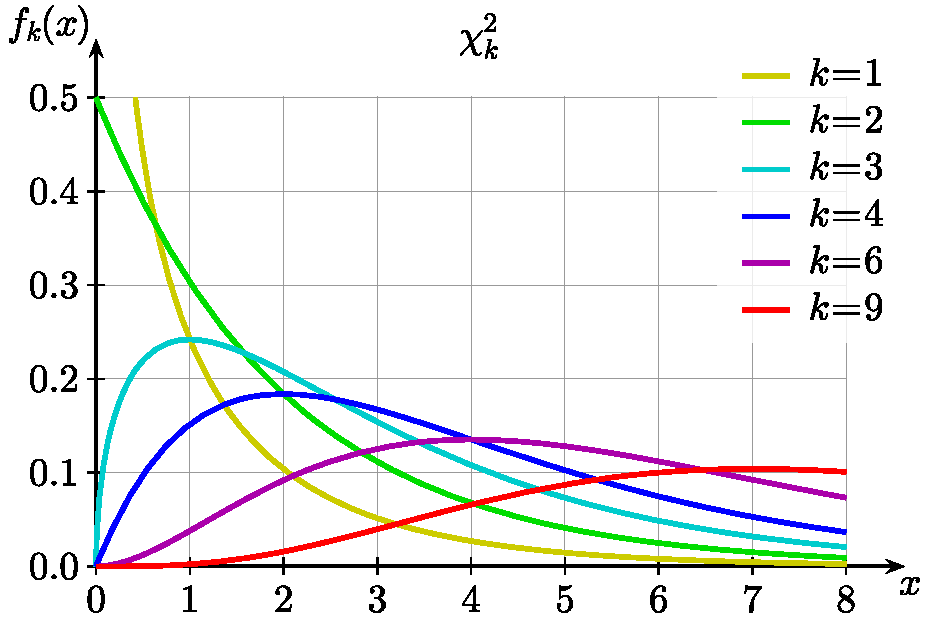
\includegraphics[width=0.7\textwidth]{../Diagrams/Chi-square.pdf}
  \caption{Illustration of how the \(\chi_{(\nu)}^2\) distribution looks with increasing degree of freedom \(\nu\).}
  \label{fig:chi-square}
\end{figure}
\begin{stbox}{General Information}
  \begin{itemize}
    \item Properties of chi-squared distributions.
    \begin{itemize}
      \item \(\E(X)=v\) and \(\Var(X)=2\nu\).
      % , and the mode of \(X\) is \(\max\{k-2,0\}\).
      \item The \(\chi_{(\nu)}^2\) distribution tends to a normal distribution as \(\nu\to\infty\).
      \item Suppose \(Z_i\sim\Normal(0,1)\) are independent. Then, \(Z_1^2+\dots+Z_n^2\sim\chi^2_{(n)}\).
      \item If \(X\sim\chi_{(\nu)}^2\) and \(Y\sim\chi_{(\upsilon)}^2\), then \(X+Y\sim\chi_{(\nu+\upsilon)}^2\).
    \end{itemize}
    \item A goodness-of-fit test.
    \begin{enumerate}
      \item Let [\(X\) in context].
      \item 
      \begin{tabular}{|ll|}
        \hline
        Test & \(H_0\colon\text{[\(X\) follows the distribution in context]}\)\\
        against &\(H_1\colon\text{[\(X\) does not follows the distribution in context]}\)\\
        \multicolumn{2}{|l|}{at the \(100\alpha\%\) significance level.}\\
        \hline
      \end{tabular}
      \item ~
      \begin{table}[H]
        \centering
        \begin{tabular}{|Sc|Sc|Sc|Sc|Sc|}
          \hline
          \(x\) & \(x_1\) & \(x_2\) & \(\cdots\) & \(x_n\)\\
          \hline
          Observed frequency \(f_i\) & \(f_1\) & \(f_2\) & \(\cdots\) & \(f_n\)\\
          \hline
          Expected frequency \(e_i\) & \(e_1\) & \(e_2\) & \(\cdots\) & \(e_n\)\\
          \hline
        \end{tabular}
        \caption{Observed and expected frequencies for a goodness-of-fit test}
        \label{table:goodness-of-fit-test}
      \end{table}
      \item Under \(H_0\), the test statistic is
      \[\chi^2=\sum_{i=1}^{n}{\frac{(F_i-E_i)^2}{E_i}}\sim\chi_{(\nu)}^2.\]
      Here, \(n\coloneq\#\text{classes}\) and \(\nu=(\#\text{classes}-\#\text{estimated parameters})-1\).
      \item Continue as per usual, calculating the critical region \(\chi_{(\nu)}^2>\chi^2_{(\nu,1-\alpha)}\) or the \(p\)-value.
    \end{enumerate}
  \end{itemize}
\end{stbox}
\begin{note}
  If \(X\) follows a \emph{discrete} normal distribution, we must state it out in words. We cannot write \(X\sim\Normal(\mu,\sigma^2)\) as this would denote that \(X\) is a \emph{continuous} random variable. 

  But if we really have \(X\sim\Normal(n,p)\) (or \(X\sim\Binom(n,p)\), \(X\sim\Poisson(\lambda)\), etc), then we can just denote it as such. 
\end{note}
\begin{note}
  The expected frequency for each of the \(n\) classes should be at least 5. If it isn't, we need to combine \emph{just enough} adjacent classes, till they do.
\end{note}
\begin{example}{\(\#\text{estimated parameters}=0\)}{}
  Given \(X\sim\Normal(0,1)\) (note how the \emph{population parameters} that define the distribution are \emph{known}), the degree of freedom \(\nu=\#\text{estimated parameters}\coloneq n\).
\end{example}
\begin{example}{\(\#\text{estimated parameters}=1\)}{}
  Consider when \(X\sim\Binom(m,p)\), such that the expected frequency for each of the \(n\) classes is at least 5, but we do not know the exact value of \(p\). So, we \emph{estimate} it according to the sample given. Then, the degree of freedom is \(\nu=n-1-1=n-2\).
\end{example}
\begin{example}{\(\#\text{estimated parameters}=2\)}{}
  Similarly, suppose \(X\sim\Normal(\mu,\sigma^2)\), such that the expected frequency of each of the \(n\) classes is at least 5, and the true value of \(\mu\) and \(\sigma^2\) are unknown. In this case, the degree of freedom \(\nu=n-2-1=n-3\). 
\end{example}
\begin{GCSkills}{}
  \begin{itemize}
    \item To find the value of \(\chi^2_{(\nu,1-\alpha)}\), which satisfies \(\Prob\left(X>\chi^2_{(\nu,1-\alpha)}\right)=\alpha\), we use the table in the \href{https://www.seab.gov.sg/docs/default-source/national-examinations/syllabus/alevel/2022syllabus/List_MF26_y22_sy.pdf}{MF26 formula sheet (Page 9)}. Unfortunately, there is no inverse \(\chi^2\) function available.
    \item For the \(p\)-value:
    \begin{center}
      \texttt{stat} \(\Longrightarrow\) \texttt{TESTS} \(\Longrightarrow\) \texttt{D:\(\chi^2\)GOF-Test\dots}
    \end{center}
  \end{itemize}
\end{GCSkills}
\begin{stbox}{}
  Tests of independence. 
  \begin{enumerate}
    \item Let [\(X\) in context].
    \item 
    \begin{tabular}{|ll|}
      \hline
      Test & \(H_0\colon\text{[\(X\) in context] is independent of [\(Y\) in context]}\)\\
      against &\(H_1\colon\text{[\(X\) in context] is dependent on [\(Y\) in context]}\)\\
      \multicolumn{2}{|l|}{at the \(100\alpha\%\) significance level.}\\
      \hline
    \end{tabular}
    \item ~
    \begin{table}[H]
      \hypertarget{table:tests-of-indepedence}{}
      \centering
      \begin{tabular}{ScSc|Sc|Sc|Sc|Sc|Sc}
        \cline{3-6}
        &&\multicolumn{4}{Sc|}{\(X\)}&\\
        \cline{3-7}
        && \(x_1\) & \(x_2\) & \(\cdots\) & \(x_n\) & \multicolumn{1}{Sc|}{Total}\\
        \cline{1-7}
        \multicolumn{1}{|Sc|}{\multirow{4}{*}{\(Y\)}}&\(y_1\)&&&&&\multicolumn{1}{Sc|}{\(t_{r_1}\)}\\ 
        \cline{2-7}
        \multicolumn{1}{|Sc|}{}&\(y_2\)&&&&&\multicolumn{1}{Sc|}{\(t_{r_2}\)}\\ 
        \cline{2-7}
        \multicolumn{1}{|Sc|}{}&\(\vdots\)&&&&&\multicolumn{1}{Sc|}{\vdots}\\
        \cline{2-7}
        \multicolumn{1}{|Sc|}{}&\(y_m\)&&&&&\multicolumn{1}{Sc|}{\(t_{r_m}\)}\\  
        \cline{1-7}
        \multicolumn{1}{Sc|}{}& Total & \(t_{c_1}\) & \(t_{c_2}\) & \(\cdots\) & \(t_{c_n}\) & \multicolumn{1}{Sc|}{\(\sum{t_{r_i}}+\sum{t_{c_i}}\)}\\ 
        \cline{2-7}
      \end{tabular}
      \caption{\emph{Expected} frequencies for a test of independence.}
      \label{table:tests-of-indepedence}
    \end{table}
    \item Under \(H_0\), the test statistic is
    \[\chi^2=\sum_{i=1}^{n}{\frac{(F_i-E_i)^2}{E_i}}\sim\chi_{(\nu)}^2.\]
    Here, \(n\coloneq\#\text{cols}\) and \(\nu=(\#\text{rows}-1)(\#\text{cols}-1)\).
    \item Continue as per usual, calculating the critical region \(\chi_{(\nu)}^2>\chi^2_{(\nu,1-\alpha)}\) or the \(p\)-value.
  \end{enumerate}
\end{stbox}
\begin{GCSkills}{}
  Key in the matrix of \emph{\textcolor{green!70!black}{observed} frequencies} (not Table \hyperlink{table:tests-of-indepedence}{\textcolor{red}{1.2}} of \emph{\textcolor{red}{expected}} frequencies): 
  \begin{center}
    \texttt{2nd} \(\Longrightarrow\) \(\texttt{x}^{-1}\) \(\Longrightarrow\) \texttt{EDIT} \(\Longrightarrow\) \texttt{[A]}.
  \end{center}
  Then, conduct the test for independence:
  \begin{center}
    \texttt{stat} \(\Longrightarrow\) \texttt{TESTS} \(\Longrightarrow\) \texttt{C:\(\chi^2\)-Test\dots}
  \end{center}
\end{GCSkills}

\chapter{Correlation and Linear Regression}
\begin{note}
  A good scatter diagram should follow the guidelines below.
  \begin{itemize}
    \item The relative position of each point on the scatter diagram should be clearly shown.
    \item The range of values for the set of data should be clearly shown by marking out the extreme \(x\) and \(y\) values on the corresponding axis.
    \item The axes should be labeled clearly with the variables.
  \end{itemize}
\end{note}
\begin{stbox}{General Information}
  \begin{itemize}
    \item The Product Moment Correlation Coefficient is a measure of the linear correlation between two variables. It is defined by
    \[r=\frac{\sum{(x-\bar{x})(y-\bar{y})}}{\sqrt{\sum{(x-\bar{x})^2}\sum{(y-\bar{y})^2}}}=\frac{\sum{xy}-\dfrac{\sum{x}\sum{y}}{n}}{\sqrt{\left[\sum{x^2}-\dfrac{\left(\sum{x}\right)^2}{n}\right]\left[\sum{y^2}-\dfrac{\left(\sum{y}\right)^2}{n}\right]}},\]
    which takes on a value from 0 to 1.
    \item When \(r=0\), there is no linear relationship. But, a nonlinear relationship may be present. Additionally, the regression lines are perpendicular.
    \item The closer the value of \(r\) is to 1 (or -1), the stronger the positive (or negative) linear correlation. Furthermore, the regression lines coincide.
    \begin{center}
      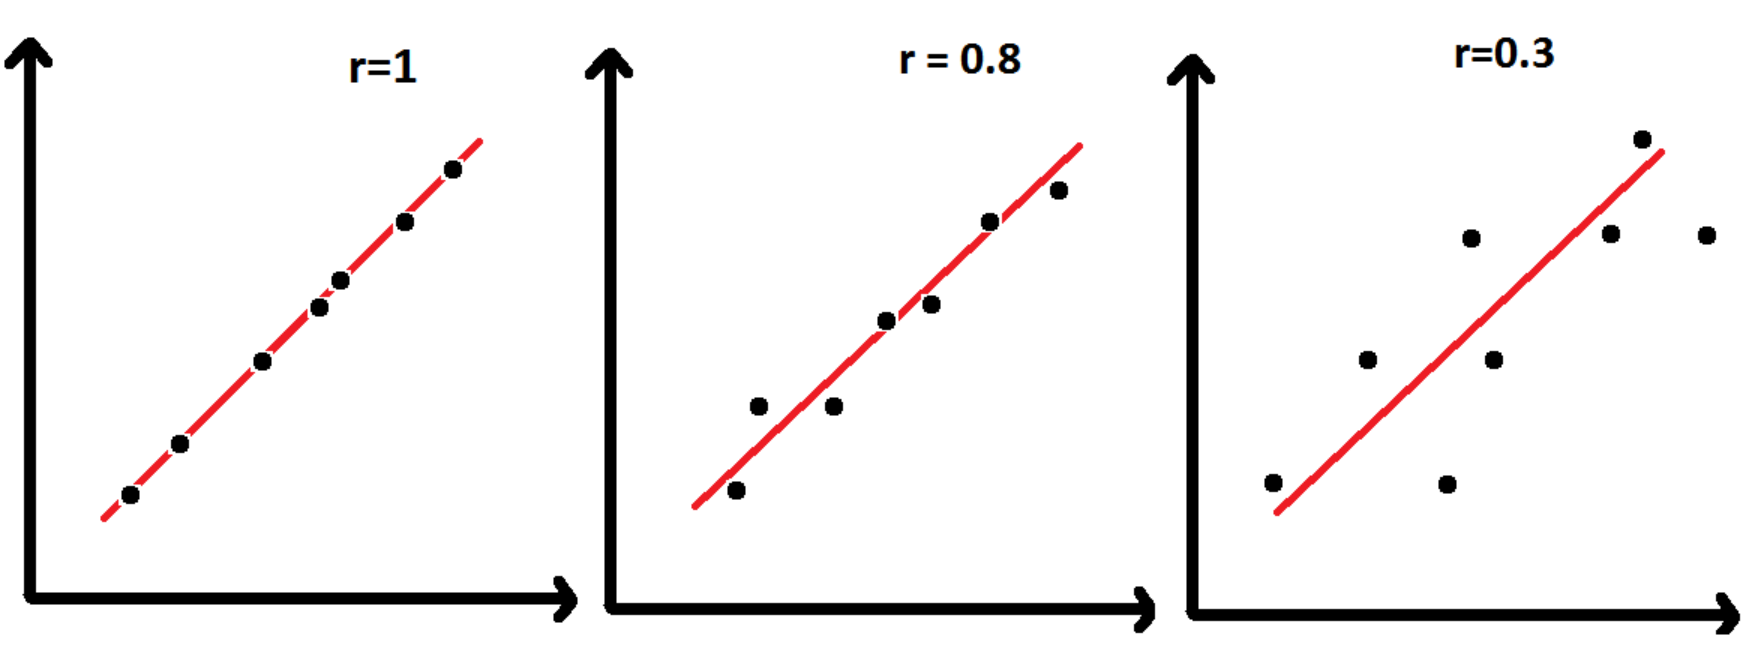
\includegraphics[scale=0.3]{../images/Product Moment Correlation Coefficient 1.png}
      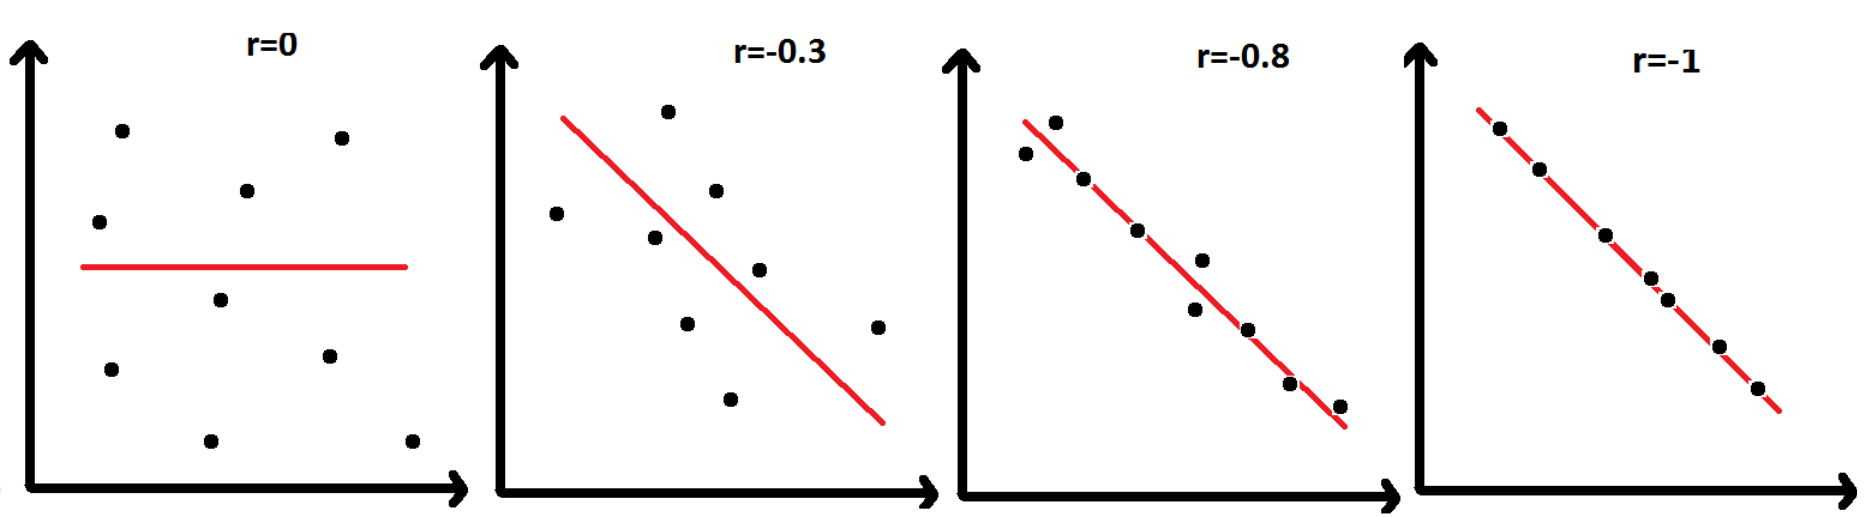
\includegraphics[scale=0.4]{../images/Product Moment Correlation Coefficient 2.png}
    \end{center}
    \item The regression line of \(y\) on \(x\) minimises the sum of squares deviation (error) in the \(y\)-direction. (i.e. we are assuming \(x\) is the independent variable whose values are known exactly.) It is given by
    \[y=\bar{y}+b(x-\bar{x}),\qquad\text{where}\qquad b=\frac{\sum{(x-\bar{x})(y-\bar{y})}}{\sum{(x-\bar{x})^2}}=\frac{\sum{xy}-\dfrac{\sum{x}\sum{y}}{n}}{\sum{x^2}-\dfrac{\left(\sum{x}\right)^2}{n}}.\] 
    \item The point \((\bar{x},\bar{y})\) always lies on both the regression lines of \(y\) on \(x\), and \(x\) on \(y\).
    \item Say we are given the value of one variable, and asked to approximate the the value of the other variable. Then, we should always use the line of the \emph{dependent} variable on the \emph{independent}.
    \item Estimations should not be taken for data outside the range of the sample provided, even if the value of \(r\) is close to 1.
  \end{itemize}
\end{stbox}
\end{document}